%!TeX root=../tese.tex

\chapter{Literatura formal}
\label{cap:literatura-formal}

\section{\citetitle{elsevier} \parencite*{elsevier}}

In particular, we studied the following five broad SE activities: (a)
implementing new features, (b) writing tests, (c) bug triaging, (d)
refactoring, and (e) writing natural-language artifacts, as well as their
individual stages. Our survey included 38 main questions, of them 5
being open-ended, which allowed the participants to freely express
their thoughts. The survey attracted 547 complete responses, and after
careful filtering, we study 481 responses. Our sample is experienced
and diverse, with almost half of the respondents having more than
10 years of professional experience covering all the major programming
languages and types of developed software.
Overall, the contributions of this work are the following:
• Usage patterns. We find that 84.2% of the respondents occasion-
ally or regularly use AI assistants, that Implementing new features
is the most popular activity to use assistants, and that among
individual stages, generating and summarizing code are the most
widely used.
• Areas of focus. Taking into account which activities the develop-
ers find less enjoyable and want to delegate, as well as what stages
AI assistants are used on, we highlight areas where the research
needs to focus on to bring value to users right now. This includes
Writing tests in general and generating data and resources for tests
in particular, as well as Writing natural language artifacts.
• Reasons for not using AI. We provide 20 distinct themes that
represent different reasons why developers are not using AI assis-
tants and report the main ones for all activities. The most popular
ones are Lack of need for AI assistance, AI-generated output being
inaccurate, User’s lack of trust and the desire to feel in control, and
Lack of understanding context by AI assistant.
• Areas of future improvement. Based on the prevalence of dif-
ferent reasons, we formulate the main areas of future work that
are needed to overcome the shortcomings that the respondents
describe. This includes the improvement of base systems, better
integration into developers’ workflow, and more actively edu-
cating and informing users about the assistants’ capabilities and
limitations.

Liang et al. [12] conducted an exploratory qualitative study on
the usage of AI programming assistants, highlighting motivations for
usage, usability challenges, and implications for creators and users of
these tools. The study had 410 developers as participants. The authors
concluded that while using AI to reduce keystrokes, finish programming
tasks quickly, and recall syntax, developers sometimes struggle to
receive AI outputs that align with their requirements and expectations.
Wang et al. [13] present a study that aims to understand practi-
tioners’ expectations on code completion, compare them with existing
research, and highlight the need for researchers to develop techniques
that meet practitioners’ demands. The methodology involves semi-
structured interviews with 15 professionals and an exploratory survey
with 599 professionals. The authors found that practitioners expect
code completion tools to work for different granularities and scenarios.
They also expect a tool to be accurate, display personalized completion,
be available offline, and be relatively fast.
Ziegler et al. [14] discuss the use of neural code synthesis in soft-
ware development and study perceived productivity by investigating
whether usage measurements of developer interactions with GitHub
Copilot can predict perceived productivity as reported by developers
in a survey. The authors found that the acceptance rate of shown
suggestions is a better predictor of perceived productivity than more
specific metrics regarding the persistence of completions in the code
over time. This suggests that the rate at which suggestions are accepted
drives developers’ perception of productivity.

Pothukuchi et al. [15] examine the potential of generative AI to
automate and enhance traditional software development practices,
thereby improving efficiency and reducing costs. A total of 30 profes-
sionals participated in the interview study and highlighted significant
improvements in development speed and code quality. The authors
indicate that generative AI can significantly transform the SDLC by
automating repetitive tasks and providing intelligent code sugges-
tions, and propose a new model called Generative AI-Assisted Software
Development Lifecycle.
Mozannar et al. [16] conducted a comprehensive study to inform
the understanding of how developers interact with AI tools and how to
improve this experience. They studied the impact of GitHub Copilot
on programmers’ behavior during coding sessions. As a result, they
identified 12 common programmer activities related to AI code comple-
tion systems. The researchers found that developers spend more time
reviewing code than writing it.

Barke et al. [17] propose a grounded theory of the bimodal nature of
programmers’ interactions with AI assistance that states that there are
two main interaction modes between which developers fluidly switch
while programming — exploration and acceleration. In acceleration
mode, the programmer already knows what they want to do next, and AI helps them get there quicker; interactions in this mode are fast and
do not break programmer’s flow. In exploration mode, the programmer
is not sure how to proceed and uses Copilot to explore their options
or get a starting point for the solution; interactions in this mode are
slow and deliberate, and include explicit prompting and more extensive
validation.

Moreover, several companies from industry conducted large-scale
studies to form an understanding of the market of AI tooling for coding.
A survey of 89,184 developers conducted in 2023 by Stack Over-
flow [9] found that 70% are using or planning to use AI tools, with 77%
expressing a favorable view. Respondents noted increased productivity
with these tools, as well as their trust in their accuracy. The most recent
Stack Overflow survey [18], conducted on 1700 people, revealed the
continuation of the trend — users report more quality work time.
A GitHub survey [19] of 500 non-manager developers found that
67% have used AI tools both at work and in personal projects. 70%
believe AI coding tools will benefit their work, primarily for upskilling
and productivity gains. 81% expect these tools to enhance team collab-
oration, particularly in security reviews, planning, and pair program-
ming.
The JetBrains Developer Ecosystem Survey [20] found that de-
velopers are optimistic about AI advancements and actively use its
capabilities despite security and ethical concerns. 59% have security
concerns, 42% ethical concerns, yet 53% are willing to use generative
AI services for work. Most commonly, developers use AI to ask gen-
eral software development questions and generate code, comments, or
documentation.

\begin{figure}[h!]
    \caption{Ferramentas utilizadas pelos desenvolvedores (\cite{elsevier}; n = 481)}
    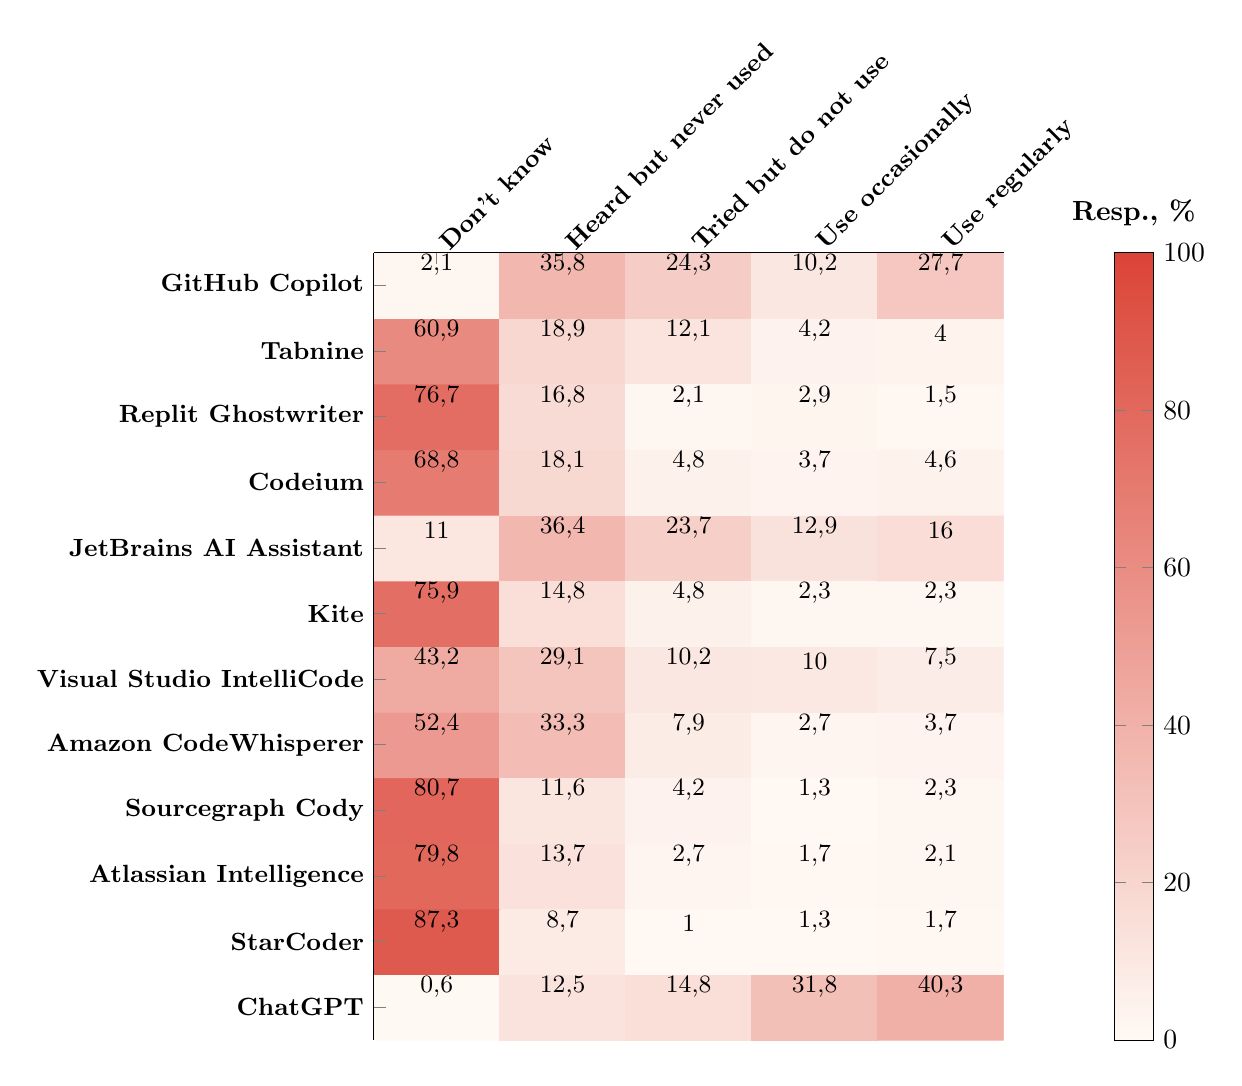
\begin{tikzpicture}
        \begin{axis}[
                /pgf/number format/use comma,
                enlargelimits=false,
                axis on top,
                scale only axis,
                width=8cm,
                height=10cm,
                xmin=0, xmax=5,
                ymin=0, ymax=12,
                xtick={0.5, 1.5, 2.5, 3.5, 4.5},
                ytick={0.5, 1.5, 2.5, 3.5, 4.5, 5.5, 6.5, 7.5, 8.5, 9.5, 10.5, 11.5},
                yticklabels={
                        ChatGPT,
                        StarCoder,
                        Atlassian Intelligence,
                        Sourcegraph Cody,
                        Amazon CodeWhisperer,
                        Visual Studio IntelliCode,
                        Kite,
                        JetBrains AI Assistant,
                        Codeium,
                        Replit Ghostwriter,
                        Tabnine,
                        GitHub Copilot
                    },
                xticklabels={
                        Don't know,
                        Heard but never used,
                        Tried but do not use,
                        Use occasionally,
                        Use regularly
                    },
                xticklabel style={
                        rotate=45,
                        anchor=west,
                        font=\bfseries\small
                    },
                yticklabel style={
                        font=\bfseries\small,
                        align=right
                    },
                axis x line*=top,
                axis y line*=left,
                colorbar,
                colorbar style={
                        title={Resp., \%},
                        title style={font=\bfseries},
                        ytick={0,20,40,60,80,100},
                        yticklabel style={font=\bfseries}
                    },
                colormap={redscale}{
                        rgb255(0cm)=(255, 250, 245);
                        rgb255(1cm)=(219, 68, 55)
                    },
                point meta min=0,
                point meta max=100,
                nodes near coords={
                        \pgfmathprintnumber[fixed, precision=1]{\pgfplotspointmeta}
                    },
                nodes near coords style={
                        font=\bfseries\small,
                        color=black
                    }
            ]
            \addplot [
                matrix plot*,
                mesh/rows=12,
                mesh/cols=5,
                point meta=explicit
            ] coordinates {
                    % ChatGPT
                    (0.5,0.5) [0.6]  (1.5,0.5) [12.5] (2.5,0.5) [14.8] (3.5,0.5) [31.8] (4.5,0.5) [40.3]
                    % StarCoder
                    (0.5,1.5) [87.3] (1.5,1.5) [8.7]  (2.5,1.5) [1.0]  (3.5,1.5) [1.3]  (4.5,1.5) [1.7]
                    % Atlassian Intelligence
                    (0.5,2.5) [79.8] (1.5,2.5) [13.7] (2.5,2.5) [2.7]  (3.5,2.5) [1.7]  (4.5,2.5) [2.1]
                    % Sourcegraph Cody
                    (0.5,3.5) [80.7] (1.5,3.5) [11.6] (2.5,3.5) [4.2]  (3.5,3.5) [1.3]  (4.5,3.5) [2.3]
                    % Amazon CodeWhisperer
                    (0.5,4.5) [52.4] (1.5,4.5) [33.3] (2.5,4.5) [7.9]  (3.5,4.5) [2.7]  (4.5,4.5) [3.7]
                    % Visual Studio IntelliCode
                    (0.5,5.5) [43.2] (1.5,5.5) [29.1] (2.5,5.5) [10.2] (3.5,5.5) [10.0] (4.5,5.5) [7.5]
                    % Kite
                    (0.5,6.5) [75.9] (1.5,6.5) [14.8] (2.5,6.5) [4.8]  (3.5,6.5) [2.3]  (4.5,6.5) [2.3]
                    % JetBrains AI Assistant
                    (0.5,7.5) [11.0] (1.5,7.5) [36.4] (2.5,7.5) [23.7] (3.5,7.5) [12.9] (4.5,7.5) [16.0]
                    % Codeium
                    (0.5,8.5) [68.8] (1.5,8.5) [18.1] (2.5,8.5) [4.8]  (3.5,8.5) [3.7]  (4.5,8.5) [4.6]
                    % Replit Ghostwriter
                    (0.5,9.5) [76.7] (1.5,9.5) [16.8] (2.5,9.5) [2.1]  (3.5,9.5) [2.9]  (4.5,9.5) [1.5]
                    % Tabnine
                    (0.5,10.5) [60.9] (1.5,10.5) [18.9] (2.5,10.5) [12.1] (3.5,10.5) [4.2]  (4.5,10.5) [4.0]
                    % GitHub Copilot
                    (0.5,11.5) [2.1]  (1.5,11.5) [35.8] (2.5,11.5) [24.3] (3.5,11.5) [10.2] (4.5,11.5) [27.7]
                };
        \end{axis}
    \end{tikzpicture}
\end{figure}

\section{\citetitle{anssi_2024} \parencite*{anssi_2024}}

O relatório foi elaborado conjuntamente pela \emph{Agence Nationale de la Sécurité des Systèmes d’Information} (ANSSI), agência francesa responsável pela cibersegurança nacional, e pelo \emph{Bundesamt für Sicherheit in der Informationstechnik} (BSI), o Escritório Federal Alemão para Segurança da Informação. Ambas são autoridades governamentais que atuam na definição de diretrizes, recomendações e boas práticas para a proteção de sistemas de informação e infraestrutura digital em seus respectivos países.

A publicação analisa as oportunidades e os riscos associados ao uso de assistentes de programação baseados em IA, tecnologia que já é amplamente adotada em organizações e tende a se tornar parte integrante do desenvolvimento de software. O relatório começa com uma introdução conceitual sobre o que são assistentes de código com IA e o objetivo do documento. Em seguida, o texto é dividido em seções temáticas que discutem, separadamente, as oportunidades associadas ao uso dessas ferramentas, os riscos de segurança envolvidos e, por fim, um conjunto de recomendações práticas. A conclusão consolida essas recomendações, segmentando-as por níveis organizacionais (gestão, desenvolvimento e pesquisa), o que confere ao texto um caráter normativo e orientado à aplicação prática, típico de publicações institucionais de órgãos de segurança da informação.

O conteúdo em detalhes do artigo não foi compilado na íntegra neste trabalho, pois é bastante denso e repleto de citações diversas. Em vez disso, seu conteúdo e suas referências serão utilizados diretamente na análise presente no \autoref{cap:analise}.